\newpage

\lecture{9}{Неравенство Брунна-Минковского.}

\subsection{Достаточное условие совпадения мер.}

\begin{remark}
    Ранее была построена <<мера с заданной функцией распределения $F$>>, то есть функция
    $\mu:\:\FB(\R)\to[0,\,+\infty]$
    такая, что
    \begin{equation}
        \label{lect9:eq:1}
        \mu((-\infty,\, a])=F(a),
    \end{equation}
    где $F:\: \R\to\R$~--- непрерывна и неубывает.
    Тогда, в силу аддитивности, $\mu((a,\,b])=\mu((-\infty,\, b])-\mu((-\infty,\, a])$.
    Откуда следует, что $\mu$, удовлетворяющая условию \eqref{lect9:eq:1}, единственна.
\end{remark}

\begin{theorem}
    Пусть $\F$~--- $\pi$"=система подмножеств множества $X$. Пусть $\mu,\, \nu:\:
        \sigma(\F)\to[0,\, +\infty]$~--- $\sigma$"=аддитивные меры, причем $\mu$ и $\nu$
    совпадают на $\F$, т. е. $\mu(A)=\nu(A)\ \forall A\in\F$.
    Пусть $\exists \{P_k\}_{k=1}^{\infty}\in\F:\: X=\bigcup\limits_{k=1}^{\infty}P_k$ и
    $\mu(P_k)=\nu(P_k)\in\R$. Тогда $\mu$ и $\nu$ совпадают на $\sigma(\F)$.

    \begin{proof}
        При доказательстве пользуемся теоремой Дынкина (\ref{theorem:dynkin}).

        Пусть сначала $X\in\F$ и меры $\mu,\, \nu$~--- конечные (для простоты).
        Обозначим
        \[
            \CE := \{A\in\sigma(\F):\ \mu(A)=\nu(A)\}.
        \]
        Заметим, что $\CE$~--- $\lambda$"=система. В самом деле, если $X\in\F$, то
        \[
            \begin{cases}
                \mu(X)=\nu(X), \\
                \mu(A)=\nu(A).
            \end{cases}\Rightarrow\mu(A^C)=\mu(X)-\mu(A)=\nu(A)-\nu(X)=\nu(A^C).
        \]
        То есть, если $A\in\CE$, то $A^C\in\CE$. Теперь докажем, замкнутость относительно взятия
        счетных дизъюнктных объединений. Пусть $A_1,\,A_2,\,\ldots\in\CE$ и попарно
        не пересекаются. Тогда \[
            \mu\left(\bigsqcup_{k=1}^{\infty}A_k\right)=\sum_{k=1}^{\infty}\mu(A_k)=
            \sum_{k=1}^{\infty}\nu(A_k)=\nu\left(\bigsqcup_{k=1}^{\infty}A_k\right).
        \]
        Откуда получаем, что $\bigsqcup\limits_{k=1}^{\infty}\in\CE$.

        Итак, $\CE$~--- $\lambda$"=система. Так как $\F\subset\CE$, то по теореме Дынкина
        $\sigma(\F)\subset \CE$, что и требовалось доказать.

        \textbf{Общий случай.} Возьмем теперь
        \[
            \CE:=\left\{A\in\sigma(\F):\: \mu\left(A\cap\bigcup_{k=1}^{n}P_k\right)=
            \nu\left(A\cap\bigcup_{k=1}^{n}P_kr\right)\right\}.
        \]
        Аналогично проверяется, что $\CE$~--- $\lambda$"=система.
        \[
            \begin{cases}
                \mu(P_1)=\nu(P_1),                 \\
                \mu(P_2)=\nu(P_2),                 \\
                \mu(P_1\cap P_2)=\nu(P_1\cap P_2). \\
            \end{cases}\Rightarrow \begin{array}{l}
                \mu(P_1\setminus P_2)   =\mu(P_1)-\mu(P_1\cap P_2)=\nu(P_1)-\nu(P_1\cap P_2)= \\
                =\nu(P_1\setminus P_2)\Rightarrow\mu(P_1\cup P_2)=\nu(P_1\cup P_2).
            \end{array}
        \]
        И аналогично доказывается, $\mu\left(\bigcup\limits_{k=1}^n P_k\right)=
            \nu\left(\bigcup\limits_{k=1}^n P_k\right)$.

        По теореме Дынкина $\sigma(\F)\subset \CE$. Тогда $\forall A\in \sigma(\F)$
        выполняется
        \[
            \mu\left(A\cap \bigcup_{k=1}^n P_k\right)=\nu\left(A\cap \bigcup_{k=1}^n P_k\right).
        \]
        Данное условие верно для любого $n\in \N$. Ранее было доказано, что если $\mu:\:
            \sigma(\F)\to[0,\,+\infty]$~--- $\sigma$"=аддитивна, то $\forall A_n\in\sigma(\F)$:
        \[
            \mu\left(\bigcup_{n=1}^{\infty}A_n\right)=\lim_{n\to\infty}
            \mu\left(\bigcup_{k=1}^n A_k\right).
        \]
        Тогда
        \[
            \mu\left(A\cap\bigcup_{k=1}^n P_k\right)\xrightarrow[n\to\infty]{}
            \mu\underbrace{\left(A\cap \bigcup_{k=1}^{\infty}P_k\right)}_{A\cap X}=\mu(A).
        \]
        И аналогично для $\nu$, то есть получаем, что $\mu(A)=\nu(A)$.

    \end{proof}
\end{theorem}

\subsection{Неравенство Брунна-Минковского.}

Пусть $\lambda$~--- мера Лебега.
\begin{lemma}
    \label{lect9:lemma:1}
    Если $K\subset\R^d$~--- компакт, то
    \[
        \lambda(K)=\lim_{\delta\to 0}\lambda(K_{\delta}),
    \]
    где $K_{\delta}=K+B_{\delta}(0)$. $B_{\delta}$~--- шарик радиуса $\delta$.

    \begin{proof}

        Покроем компакт не шариками, а клетками размера $\delta$. На прошлых лекциях
        было доказано, что
        \[
            \lambda(K)=\inf\{\lambda(U)\ \mid\ U\subset \R^d\text{ открыто},\ K\subset U\}.
        \]
        Возьмем открытое множество, которое покрывает данный компакт: $\forall\varepsilon>0
            \ \exists\text{открытое }U:\: \lambda(U)<\lambda(K)+\varepsilon$.
        Тогда $\exists\delta_1>0:\ K_{\delta}\subset U\text{ при }\delta<\delta_1
            \Rightarrow\lambda(K)\leqslant\lambda(K_{\delta})
            \leqslant\lambda(U)<\lambda(K)+\varepsilon\ \forall\delta\in(0,\, \delta_1)$.

        \begin{remark}
            Такое $\delta_1$ найдется, потому что пусть $f(x)=\rho(x,\, U^C)>0\ \forall x\in K$.
            Тогда $f$~--- непрерывна, следовательно $\exists x_0\in K:\ f(x_0)=\inf\limits_{x\in K}
                f(x)\Rightarrow\delta_1=f(x_0)$.
        \end{remark}

    \end{proof}
\end{lemma}

\begin{theorem}[неравенство Брунна-Минковского]
    Пусть $A,\, B\subset \R^d$~--- компакты. Тогда
    \begin{equation}
        \label{lect9:eq:2}
        \lambda^{1/d}(A+B)\geqslant \lambda^{1/d}(A)+\lambda^{1/d}(B),
    \end{equation}
    где $A+B=\{a+b\ \mid\ a\in A,\, b\in B\}$~--- сумма Минковского.

    \begin{proof}
        Пусть вначале
        \[
            \begin{array}{ll}
                A=I_1\times I_2\times\ldots\times I_d,\quad & m(I_k)=\alpha_k> 0, \\
                B=J_1\times J_2\times\ldots\times J_d,\quad & m(J_k)=\beta_k> 0.
            \end{array}
        \]
        Отмасштабируем множества $A$ и $B$ так, чтобы $\alpha_k+\beta_k=1$, понятно, что при этом
        неравенство \eqref{lect9:eq:2} не изменится.

        Распишем сумму Минковского:
        \[
            A+B=(I_1+J_1)\times(I_2+J_2)\times\ldots\times(I_d+J_d).
        \]
        И за счет масштабирования имеем: $\lambda(A+B)=1$.
        Теперь распишем меры $A$ и $B$:
        \[
            \begin{array}{l}
                \lambda(A)=\alpha_1\cdot\alpha_2\cdot\ldots\cdot\alpha_d, \\
                \lambda(B)=\beta_1\cdot\beta_2\cdot\ldots\cdot\beta_d.
            \end{array}
        \]
        Возведем обе части в степень $\frac{1}{d}$ и воспользуемся неравенством о среднем:
        \[
            \begin{array}{l}
                \lambda^{1/d}(A)=(\alpha_1\cdot\alpha_2\cdot\ldots\cdot\alpha_d)^{1/d}
                \leqslant\dfrac{\alpha_1+\alpha_2+\ldots+\alpha_d}{d}, \\
                \lambda^{1/d}(B)=(\beta_1\cdot\beta_2\cdot\ldots\cdot\beta_d)^{1/d}
                \leqslant\dfrac{\beta_1+\beta_2+\ldots+\beta_d}{d}.
            \end{array}
        \]
        Откуда получаем:
        \[
            \lambda^{1/d}(A)+\lambda^{1/d}(B)\leqslant\dfrac{(\alpha_1+\beta_1)+
                (\alpha_2+\beta_2)+\ldots+(\alpha_d+\beta_d)}{d}=1.
        \]
        То есть теорема доказана для случая, когда $A,\, B$~--- клетки.

        Пусть теперь $A$ и $B$~--- элементарные множества. То есть
        \[
            A = \bigsqcup_{k=1}^p A_k,\, B = \bigsqcup_{k=1}^q B_k,\quad
            \text{ где } A_k,\, B_k\text{~--- клетки}.
        \]

        Докажем индукцией по $n:=p+q$ неравенство \eqref{lect9:eq:2}.

        База индукции~--- очевидна: при $n=1$ одно из объединений пусто и неравенство вырождается
        в тривиальное.

        Без ограничения общности пусть $p>q$.
        Вспомним, что
        \[
            I_1\times \ldots\times I_d\cap J_1\times \ldots\times J_d = \varnothing
            \Leftrightarrow \exists s\in\overline{1,\, d}:\: I_s\cap J_s=\varnothing.
        \]

        \begin{center}
            

\tikzset{every picture/.style={line width=0.75pt}} %set default line width to 0.75pt        

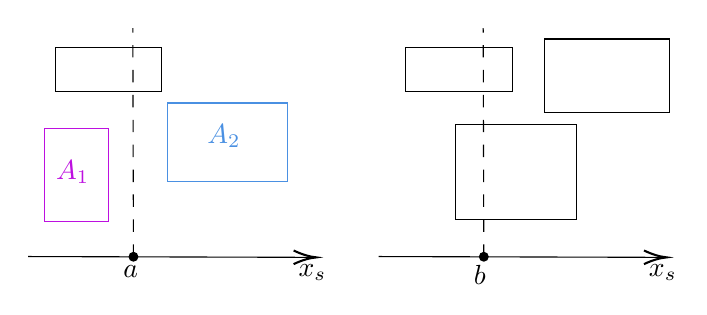
\begin{tikzpicture}[x=0.75pt,y=0.75pt,yscale=-1,xscale=1]
%uncomment if require: \path (0,300); %set diagram left start at 0, and has height of 300

%Straight Lines [id:da43900000406433426] 
\draw    (20.2,160.2) -- (157,160.59) ;
\draw [shift={(159,160.6)}, rotate = 180.17] [color={rgb, 255:red, 0; green, 0; blue, 0 }  ][line width=0.75]    (10.93,-3.29) .. controls (6.95,-1.4) and (3.31,-0.3) .. (0,0) .. controls (3.31,0.3) and (6.95,1.4) .. (10.93,3.29)   ;
%Flowchart: Connector [id:dp7933572805012272] 
\draw  [fill={rgb, 255:red, 0; green, 0; blue, 0 }  ,fill opacity=1 ] (68.8,160.3) .. controls (68.8,159.14) and (69.74,158.2) .. (70.9,158.2) .. controls (72.06,158.2) and (73,159.14) .. (73,160.3) .. controls (73,161.46) and (72.06,162.4) .. (70.9,162.4) .. controls (69.74,162.4) and (68.8,161.46) .. (68.8,160.3) -- cycle ;
%Straight Lines [id:da4965385643125464] 
\draw  [dash pattern={on 4.5pt off 4.5pt}]  (70.9,160.3) -- (70.6,50.2) ;
%Shape: Rectangle [id:dp9200245535491574] 
\draw  [color={rgb, 255:red, 189; green, 16; blue, 224 }  ,draw opacity=1 ] (28,98.6) -- (59,98.6) -- (59,143.4) -- (28,143.4) -- cycle ;
%Shape: Rectangle [id:dp13850850463841335] 
\draw  [color={rgb, 255:red, 74; green, 144; blue, 226 }  ,draw opacity=1 ] (87.2,86.2) -- (145,86.2) -- (145,124.2) -- (87.2,124.2) -- cycle ;
%Shape: Rectangle [id:dp643515768425587] 
\draw   (33.2,59.4) -- (84.6,59.4) -- (84.6,80.8) -- (33.2,80.8) -- cycle ;
%Straight Lines [id:da07346645219463133] 
\draw    (189,160.2) -- (325.8,160.59) ;
\draw [shift={(327.8,160.6)}, rotate = 180.17] [color={rgb, 255:red, 0; green, 0; blue, 0 }  ][line width=0.75]    (10.93,-3.29) .. controls (6.95,-1.4) and (3.31,-0.3) .. (0,0) .. controls (3.31,0.3) and (6.95,1.4) .. (10.93,3.29)   ;
%Flowchart: Connector [id:dp01440971299286109] 
\draw  [fill={rgb, 255:red, 0; green, 0; blue, 0 }  ,fill opacity=1 ] (237.6,160.3) .. controls (237.6,159.14) and (238.54,158.2) .. (239.7,158.2) .. controls (240.86,158.2) and (241.8,159.14) .. (241.8,160.3) .. controls (241.8,161.46) and (240.86,162.4) .. (239.7,162.4) .. controls (238.54,162.4) and (237.6,161.46) .. (237.6,160.3) -- cycle ;
%Straight Lines [id:da3918400356510574] 
\draw  [dash pattern={on 4.5pt off 4.5pt}]  (239.7,160.3) -- (239.4,50.2) ;
%Shape: Rectangle [id:dp7954809732017523] 
\draw   (202,59.4) -- (253.4,59.4) -- (253.4,80.8) -- (202,80.8) -- cycle ;
%Shape: Rectangle [id:dp5319987981150394] 
\draw   (226,96.6) -- (284.2,96.6) -- (284.2,142.2) -- (226,142.2) -- cycle ;
%Shape: Rectangle [id:dp544533004742412] 
\draw   (268.8,55.4) -- (329,55.4) -- (329,90.6) -- (268.8,90.6) -- cycle ;

% Text Node
\draw (149.2,162.6) node [anchor=north west][inner sep=0.75pt]   [align=left] {$\displaystyle x_{s}$};
% Text Node
\draw (64.8,163.2) node [anchor=north west][inner sep=0.75pt]   [align=left] {$\displaystyle a$};
% Text Node
\draw (32.4,112.6) node [anchor=north west][inner sep=0.75pt]  [color={rgb, 255:red, 189; green, 16; blue, 224 }  ,opacity=1 ] [align=left] {$\displaystyle A_{1}$};
% Text Node
\draw (105.2,95.4) node [anchor=north west][inner sep=0.75pt]  [color={rgb, 255:red, 74; green, 144; blue, 226 }  ,opacity=1 ] [align=left] {$\displaystyle A_{2}$};
% Text Node
\draw (318,162.6) node [anchor=north west][inner sep=0.75pt]   [align=left] {$\displaystyle x_{s}$};
% Text Node
\draw (233.6,163.2) node [anchor=north west][inner sep=0.75pt]   [align=left] {$\displaystyle b$};


\end{tikzpicture}

        \end{center}

        Тогда $\exists a\in\R: I_s\subset (-\infty,\, a)$ и $J_s\subset [a,\, +\infty)$ (либо наоборот, но это неважно).
        То есть найдется точка $a$, разделяющая клетки $A_k$ (см. рисунок выше).
        Снова не уменьшая общности считаем, что $s=1$. Введем теперь множества ($b$ выберем позже):
        \begin{align*}
            A^+:=A\cap \{x\in\R^d: x_1\geqslant a\}, \\
            A^-:=A\cap \{x\in\R^d: x_1<a\},          \\
            B^+:=B\cap \{x\in\R^d: x_1\geqslant b\}, \\
            B^-:=B\cap \{x\in\R^d: x_1< b\}.
        \end{align*}
        Тогда
        \[
            A+B=(A^+\sqcup A^-)+(B^+\sqcup B^-)\supset (A^++B^+)\cup(A^-+B^-),
        \]
        причем $(A^++B^+)\cap(A^-+B^-)=\varnothing$, так как
        \begin{align*}
            A^++B^+\subset \{x\in\R^d:\ x_1\geqslant a+b\}, \\
            A^-+B^-\subset \{x\in\R^d:\ x_1< a+b\}.
        \end{align*}
        То есть $A+B\supset (A^++B^+)\sqcup(A^-+B^-)$, следовательно
        \[
            \lambda(A+B)\geqslant
            \lambda((A^++B^+)\sqcup(A^-+B^-))=
            \lambda(A^++B^+)+\lambda(A^-+B^-).
        \]
        В силу предположения индукций
        \begin{align*}
            \lambda^{1/d}(A^++B^+)\geqslant\lambda^{1/d}(A^+)+\lambda^{1/d}(B^+), \\
            \lambda^{1/d}(A^-+B^-)\geqslant\lambda^{1/d}(A^-)+\lambda^{1/d}(B^-).
        \end{align*}

        Итак,
        \begin{align*}
            \lambda(A+B) & \geqslant
            \lambda(A^++B^+)+\lambda(A^-+B^-)\geqslant                                    \\
                         & \geqslant\left(\lambda^{1/d}(A^+)+\lambda^{1/d}(B^+)\right)^d+
            \left(\lambda^{1/d}(A^-)+\lambda^{1/d}(B^-)\right)^d\text{\circled{$=$}}
        \end{align*}
        Так как $A^+$ меньше $A$ хотя бы на одну клетку, то $0<\lambda(A^+)<\lambda(A)$.
        Обозначим $\theta =\dfrac{\lambda(A^+)}{\lambda(A)}\in(0,\,1)$.

        Точку $b$ выберем так, что $\dfrac{\lambda(B^+)}{\lambda(B)}=\theta$ (существование
        такой точки следует из теоремы о промежуточном значении~--- при движении
        точки $b$ вправо мера $B^+$ уменьшается). То есть разделим $B$ в таком же отношении, в
        котором $a$ делит $A$. Используя новое обозначение, можем записать
        \begin{align*}
             & \lambda(A^+)=\theta\lambda(A),     \\
             & \lambda(B^+)=\theta\lambda(B),     \\
             & \lambda(A^-)=(1-\theta)\lambda(A), \\
             & \lambda(B^-)=(1-\theta)\lambda(B).
        \end{align*}

        Продолжим равенство выше:
        \begin{align*}
             & \text{\circled{$=$} }\theta\cdot\left(\lambda^{1/d}(A)+\lambda^{1/d}(B)\right)^d
            +(1-\theta)\cdot\left(\lambda^{1/d}(A)+\lambda^{1/d}(B)\right)^d=                   \\
             & =\left(\lambda^{1/d}(A)+\lambda^{1/d}(B)\right)^d\text{, т. е. }
            \lambda^{1/d}(A+B)\geqslant \lambda^{1/d}(A)+\lambda^{1/d}(B).
        \end{align*}

        Итак, теперь доказали теорему для элементарных множеств.

        Для доказательства для компактов воспользуемся леммой \ref{lect9:lemma:1}.
        Пусть теперь $A,\, B\subset \R^d$~--- компакты.
        $\forall \varepsilon>0\ \exists$ элементарные
        $A_1,\, B_1:\ A\subset A_1,\, B\subset B_1$:
        \begin{align*}
            &\lambda^{1/d}(A_1)<\lambda^{1/d}(A)+\varepsilon, \\
            &\lambda^{1/d}(B_1)<\lambda^{1/d}(B)+\varepsilon.
        \end{align*}
        Пусть также $A_1=\bigsqcup\limits_{k=1}^p Q_k\text{~--- клетки},\,\diam Q_k<\dfrac{\delta}{2}$ 
        (и аналогично для $B_1$).
        Тогда существует $B_{\delta/2}$~--- шар радиуса $\dfrac{\delta}{2}$ такой,
        что $A\subset A_1\subset B_{\delta/2}$ и $B\subset B_1\subset B_{\delta/2}$.
        Тогда можно записать 
        \[
            A_1+B_1=(A+B_{\delta/2}(0))+(B+B_{\delta/2}(0))\subset A+B+B_{\delta}(0)=(A+B)_{\delta}.
        \]

        Итак, 
        \[
            \lambda^{1/d}(A)+\lambda^{1/d}(B)\leqslant
            \lambda^{1/d}(A_1)+\lambda^{1/d}(B_1)\leqslant
            \lambda^{1/d}(A_1+B_1)\leqslant
            \lambda^{1/d}((A+B)_{\delta})\to \lambda^{1/d}(A+B),
        \]
        в силу леммы, так как $A+B$~--- компакт. 

    \end{proof}
\end{theorem}

